% Change to 'masters' to produces the masters thesis preliminary pages
\documentclass[oneside,masters,etd]{WSUclass}

\usepackage{import}

% preamble contains title page, signature page, acknowledgment and abstract texts
\usepackage{preamble}
\usepackage{bm}

% Pacakges used
\usepackage[utf8]{inputenc} % Remove warning on ascii conversion
\usepackage[T1]{fontenc} % Remove warning on ascii conversion
\usepackage[refsection=part,citestyle=apa,style=authoryear,natbib=true,backend=biber]{biblatex}
\usepackage{hyperref}

% Make chapter numbers into string words 1 -> ONE
\usepackage{fmtcount}
\makeatletter
\renewcommand{\@makechapterhead}[1]{\vspace *{40\p@ }{\parindent \z@ 
\raggedright \normalfont \ifnum \c@secnumdepth >\m@ne \Huge \bfseries 
\@chapapp \space \Numberstring{chapter} \vskip 10\p@ \fi #1\par \nobreak \vskip 30\p@ }}
\makeatother

\addbibresource{bib.bib}

\newcommand\nt[1]{\textcolor{blue}{#1}}

\begin{document}

\hypersetup{breaklinks=true}

 % Start page counting in roman numerals
 \frontmatter

 % This command makes the formal preliminary pages.
 % You can comment it out during the drafting process if you want to save paper.
 %\makepreliminarypages

 \doublespace
 % Make the table of contents.
 \tableofcontents
 \thispagestyle{plain}

 % Make the list of tables
 \mylistoftables
 \thispagestyle{plain}
 
 % Make the list of figures
 \mylistoffigures
 \thispagestyle{plain}

  % This page is OPTIONAL. To remove, comment out and \dedicationpage in diss.tex
 %\dedicationpage
 \clearemptydoublepage

 % Start regular page counting at page 1
 \mainmatter

% OK. Everything is set up. Type your thesis here.
\addchapheadtotoc
\chapter{Context and related works}

In this chapter, we first introduce graphs and how they arise from real world networks. Then we present the graph classification problem, along with applications in which it arises. Finally, we proceed to detailing state-of-the-art methods and their limitations, before stating our contribution. 
 
\section{Graph structures and its presence in real world}

The need for graphs and their analysis can be traced back to 1679, when G.W.  Leibniz  wrote to C. Huygens about the limitations of traditional analysis methods of geometric figures and said that "we need yet another kind of analysis, geometric or linear, which deals directly with position, as algebra deals with magnitude", \citep{Graph_application}. This lead to graphs, mathematical objects that provide a pictorial and efficient form to represent data with many inter-connections. %With graph structures, these data become easier to be processed and analyzed, and that helps solving many problems that have been unsolved before \citep{Graph_application}.

Formally, a graph of size $v$ is a pair $\mathcal{G}=(\mathcal{V},\mathcal{E})$, where $\mathcal{V}=\{u_1,...,u_v\}$ is a set of $v$ graph nodes (or vertices), and $\mathcal{E}\in \mathcal{V}\times \mathcal{V}$ is the set of edges between these nodes, i.e. $(u_i, u_j)\in \mathcal{E}$ means that the graph has an edge between node $u_i$ and node $u_j$.

Graph structures are used to model a set of objects and their interactions/relations. % that link between different pairs of these objects.  
While the nature of these objects and their interactions vary with the application, the underlying modeling paradigm is the same for all applications: objects are represented by nodes, and a relation between two objects is represented by an edge between the corresponding two nodes. \nt{**For instance, in a social network like Facebook, nodes are .. and edges are... In a biological network such as the brain, nodes are brain regions and edges are.. In a transportation network such as the subway, nodes are .. and edges are.. (see Table.\ref{table:Graph_examples} for a list of different examples). } 

These graphs, if not too large, can be visually represented in order to provide an intuitive understanding of the existing interactions. Such an illustration is in Fig. \ref{fig:Graph_Example} in the application of chemical reactions.



\begin{figure}[H]
\centering
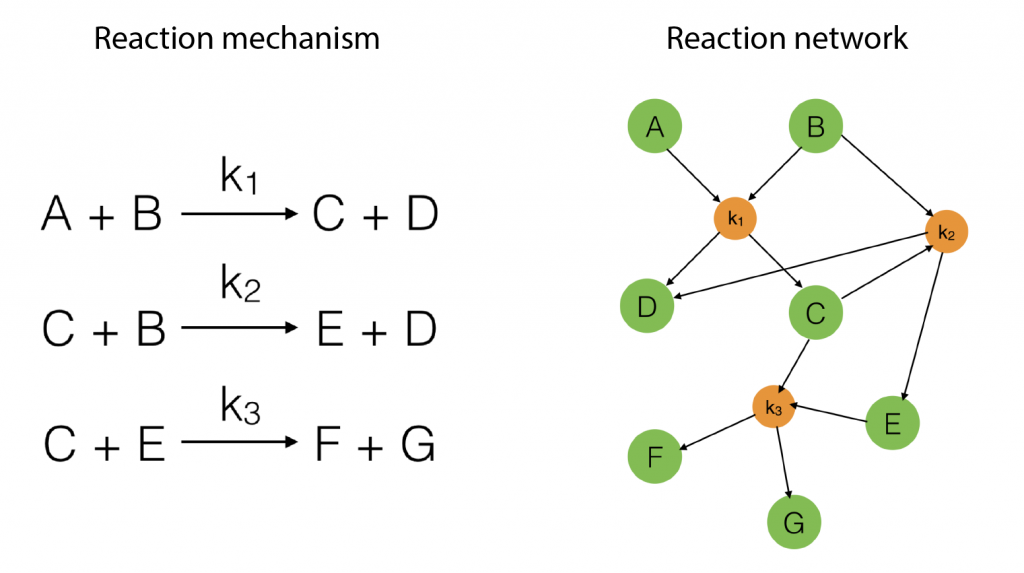
\includegraphics[scale=0.2]{figs/Graph_example.png}
\caption[Graph example to represent Chemical Reactions]{Graph structures in representing chemical reactions mechanisms}
%Source:
\label{fig:Graph_Example}
\end{figure}


\begin{table}
\small
\begin{center}
\begin{tabular}{|c|c|c|c|c|}
\hline
{Network}  &  {Nodes} & {Node features}  & {Edges}  & {Edge features}  \\
\hline
{Transportation System}  &  {cities} & {registered cars}  & {Routes}  & {Length, cost }  \\
\hline
{Banking Network}  &  {Account holders} & {account status}  & {Transactions}  & {Transaction value}  \\
\hline
{Social Network}  &  {users} & {name, country}  & {Interactions}  & {type (like, comment)}  \\
\hline
\end{tabular}
\end{center}
\caption{Some real world graphs}
\label{table:Graph_examples}
\end{table}

\section{Graph classification problem}
\label{sec:Graph_classification_problem}
Graph classification can be understood in several ways. Here, we place ourselves in the context of \emph{supervised learning}, where we suppose we have access to a set of pre-labeled graphs  $(\mathcal{X}=\{\mathcal{G}_1,\ldots,\mathcal{G}_n\}, \mathcal{Y}=\{y_1,\ldots,y_n\})$, where each graph $\mathcal{G}_i$ is \emph{a priori} known to belong to the class with label $y_i$. Stated simply, the graph classification problem we are interested in in this work may be stated as: given this prior information, design a classification algorithm that, given in input any graph (importantly, any graph belonging or not to $\mathcal{X}$), outputs the label of the class to which it belongs. 

More formally, consider the set $\mathcal{D}$ of all graphs $\mathcal{G}$ that can occur in some real-world application, a fixed set of classes $\beta=\{\beta _1,\ldots,\beta _l\}$ of finite size $l$, and a mapping function $f:\mathcal{D}\mapsto\beta$ which maps each graph $\mathcal{G}$ in $\mathcal{D}$ to the class $\beta_\mathcal{G}$ it belongs to. Graph classification is the problem of estimating the mapping function $f$ in the case where it is only known on a subset $\mathcal{X}\subset \mathcal{D}$. Formally, we have a dataset $(\mathcal{X}=\{\mathcal{G}_1,\ldots,\mathcal{G}_n\}, \mathcal{Y}=\{y_1,\ldots,y_n\})$ of size $n$ such that $\mathcal{X}\in \mathcal{D}^n$ and $\mathcal{Y}\in\beta^n$, where for each graph $\mathcal{G}_i\in \mathcal{X}$ we have that $y_i=f(\mathcal{G}_i)$ is the class of $\mathcal{G}_i$. The classification task is to have a \textbf{predictive model} which can predict well, based on some-predefined metric,  the class for any new graph $\mathcal{G}$ in $\mathcal{D}$. This prediction functionality of the model is gained using the dataset $(\mathcal{X}, \mathcal{Y})$ to optimize the parameters of the model that is believed to govern the behavior of the mapping function $f$ on $\mathcal{D}$. This optimization completed in this paradigm is called the learning algorithm.

Note that graph classification as considered here, has nothing to do with the more common problem of \emph{node classification} in a graph, in which there exists only one graph and the goal is to separate the node set in a partition of communities. In our work, graphs are classified, not nodes. This being said, the extra information that the nodes and/or edges may have in some applications (gender, age for instance for nodes of a social network; maximum bandwidth, number of channels for instance for edges of a communication network; etc.) could in principle be used along with the graph structure to classify different graphs into different classes. However, as the existence of such extra-information is very application-dependent, we prefer to focus here on the case where nodes and edges do not carry such information: the only information one has access to for classification is the graph structure.

This problem has been addressed in many different fields of research, such as:
\begin{itemize}
    \item \textbf{\emph{Marketing analytics:}} advertisers and marketers  are interested in detecting the influential people communities in Social Networks in the sense that addressing their products' advertisements to such groups would be a more rewarding investment. This can be approached with graph classification applied on these networks \citep{marketing_analytics}.
    \item \textbf{\emph{Banking security:}} graph classification is used to catch unusual patterns of fraudulent transactions \citep{banking_security}.
    \item \textbf{\emph{Biology and genomics:}} graphs are based on proteins such that nodes correspond
to amino acids which compound the protein and a pair of amino acids are linked by an edge if they are less than 6 Angstroms apart. The task is to detect whether a protein is an enzyme or not \citep{protein_application}, to mention a few.
\end{itemize}

\section{State-of-the-art methods for graph classification}
\label{section:state}
We  present here existing algorithms for the graph classification problem and discuss their limitations. In general, these algorithms can be classified in four main categories: set based, frequent sub-graph based, kernel based, and graph neural networks based algorithms.\\

\noindent\textbf{Set based algorithms.} This type of algorithms is only applicable to cases where nodes/edges are supplied with features or attributes, as they completely disregard the graph's structure. Based on the provided feature vectors, a distance function of interest between the graphs is computed. % in order to provide a similarity between pairs of edges/nodes in the corresponding sets. 
The drawback of this method is that it does not take the structure (topology) of the graph itself into consideration. For example, if we just compare how much the edges' features of one graph are similar to the edges' features of another, we can have two graphs with the same set of edge features, which will lead to maximum similarity, even though their graph structures can be arbitrarily different. %but we in reality ignore other important information that can make these graphs completely different. % such as how many connected communities of nodes these edges form in each graph, how many circles of nodes these edges promote in each graph, etc. 
On the other hand, a strength of these algorithms is their low computations cost that is usually linear or quadratic in the number of nodes and edges \citep{graphlet_kernel}.\\
 
\noindent\textbf{Frequent sub-graph based algorithms.} These algorithms contain two steps. First, the graph dataset $\mathcal{X}$ is analyzed to enumerate the frequent sub-graphs occuring in the different graphs. Then, another analysis is done to choose the most discriminative sub-graphs out of the ones found during the first step. The disadvantage of using this method is the computational cost that grows exponentially with the graph size \citep{graphlet_kernel}. \\

\noindent\textbf{Graph kernels based algorithms.} It is a middle ground between both previous methodologies, where the graph structure is well considered, and in most cases, these algorithms are designed in a way that the computational time is a polynomial function of the graph size \citep{graphlet_kernel}. However, some effective and competitive kernels still require exponential time, and this is in short the problem we approach in this work using random features to approximate these kernels or to compete with them in notably lower computational time. \\

\noindent\textbf{Graph neural networks (GNNs) based algorithms.} GNNs compute a representation vector (embedding vector) for every node in a graph, where this vector is recursively computed by aggregating the representation vectors of neighboring nodes. The goal of this aggregation technique is that nodes that are neighbors (or close) to each other in the graph are more likely to have similar representations (with respect to some similarity function) and vice versa. On the graph level, a representation vector is computed by aggregating its nodes' representation vectors. This aggregated vector now representing the graph itself is used as a usual feature vector which can be fed to a typical deep neural network to learn the classification task. Traditional GNNs such as graph convolutional networks (GCNs) and GraphSAGE fail to provide high performance classifying graphs whose node/edges don't include any original feature vectors, and that even applies on graphs with simple topology \citep{GCN_powerful}. \nt{I could not re-write this last sentence: I don't understand it} 
However, another GNN structure was developed to overcome this weakness point \nt{complete failure is more than a ``weakness''}, and it is referred to by Graph Isomorphism Network (GIN). Regarding the computational time, it is mainly a matter of the layers number in the network, since this parameter in reality represents how far from a node we want to go in order to compute its representation vector. 

\section{Our contribution}
One of the methods of the kernel-based algorithms (the third out of the four categories listed), called graphlet kernel, has proven to be competitive for graph classification. Theoretically and empirically, it was shown that a desired performance or a required amount of information to be preserved from the original graph can be reached with sufficiently large $k$. \nt{**hold your horses! we need at least a few sentences actually \emph{explaining} what is the graphlet kernel you are talking about. For instance, we have yet no clue what $k$ is.**}
However,  the computational cost  becomes prohibitive as $k$ (the graphlet size) and/or $v$ (the size of the graph)  become too large. Thus it cannot be applied on large-scale graph datasets. 

The advent of Optical Processing Units (OPUs) opened a new horizon solving this problem, since it can apply enormous number of \emph{Random Projections} in light speed. \nt{**hold your horses! The reader has no clue \emph{why} making random projections in light speed is actually useful for your problem. You need at least one sentence explaining what you mean by random projections}

In this work, we did the sufficient mathematical analysis to prove that OPUs' light-speed random feature projections compete the $k$-graphlet kernel with respect to \emph{Maximum Mean Discrepancy (MMD)} Euclidean metric. Moreover, we empirically tested this hypothesis and made sure that the the theoretical MMD error is aligned with the empirical one with respect to the parameters introduced in the problem (sampling technique, number of sampled sub-graphs, number of random features, etc). \nt{Instead of this last paragraph, I invite you to write ``Our contributions are the following:'' followed by an ``enumerate'' environment to make a clear and thorough list of your achievements. After that enumeration, I invite you to write ``On top of these contributions, we have also:'' followed by an ``enumerate'' environment to make a list of things you did that we cannot call ``contributions'' yet as they either did not work or are work in progress.}






%\include{chapter1/ch1}
\include{chapter1/chp1_NT}
\chapter{Fast graph kernel classifier based on optical random features }
\label{chapter:fast_algorithm}
\newtheorem{lemma}{Lemma} 
The graphlet kernel $\K$ is a good method to solve the graph classification problem but as we have seen in chapter \ref{chapter:background}, it suffers from a high computational cost. In this chapter, we take inspiration from it to propose a family of fast graph kernels that generalizes the graphlet kernel paradigm. We show how random features can be incorporated within the new framework to get a faster and competitive algorithm in graph classification. Finally, we describe how Optical Processing Units (OPUs) can be used to eliminate some significant computational cost altogether.

\section{Proposed algorithm}
\label{alg:GSA}
We recall from chapter \ref{chapter:background} that the computational cost of computing the $k$-spectrum $\mathbf{f}_\G$ of a graph $\G$, which is the building block of the graphlet kernel method, is $C_{gk}= O(\tbinom{v}{k} N_k C_k^{\cong})$. As an attempt to lower this cost, using random graph sampling, we can compute an approximation of the $k$-spectrum vector in time $C_{gk + gs}= O(C_S s N_k C_k^{\cong})$. We can see that $\tbinom{v}{k}$ is replaced with $C_S s$, and recall that the number of samples $s$  should scale as $N_k$ in order to ensure a reasonable estimation of $\mathbf{f}_\G$. It is clear then that to further decrease this cost, one needs to work on the time to apply $\varphi_k^{match}$ to a given graphlet, denoted by $C_{\varphi_k^{match}}=O(N_k C_k^{\cong})$.

To this end, we propose to replace $\varphi^{match}_k$ with another user-defined function $\varphi:\mathfrak{H} \mapsto\R^m$ and keep everything else as it is. We obtain a family of algorithms referred to as Graph Sampling and Averaging (GSA-$\varphi$), described in Alg.~\ref{alg:GSA}, whose main user-defined methods are the samping method $S_k$ and the feature map $\varphi$.

For a set $\mathfrak{F} = \{F_1,\ldots, F_s\}$ and a feature map $\varphi$, similarly to ${\varphi}^{hist}$ we define ${\varphi}(\mathfrak{F}) = \frac{1}{s} \sum_{F\in\mathfrak{F}} \varphi(F)$. The GSA-$\varphi$ algorithm computes, for each graph $\G$ in the dataset, an embedding ${\varphi}(\mathfrak{F}_\G)$ where $\mathfrak{F}_\G$ is a set of $s$ subgraphs drawn $iid$ from $S_k(\G)$, then trains a classifier on it.

Importantly, note that Algorithm GSA-$\varphi$ with the choices $\varphi\leftarrow\varphi^{match}_k$ and uniform sampling for $S_k$ boils down to computing the graphlet kernel $\K$ detailed in the previous chapter. Any other choice leads to something else, that might not even be an approximation of $\K$, but that still hopefully captures relevant information from the graphs in the dataset $\mathcal{X}$ enabling efficient and high-performance classification. In this sense, GSA-$\varphi$ is a generalization of the graphlet kernel method. 

\begin{algorithm}[t]
	
\DontPrintSemicolon
  \KwInput{2-Classes labelled graph dataset $\mathcal{X}=(\G_i,y_i)_{i=1,\ldots,n}$}
  \KwOutput{Trained model to classify graphs}
  \tools{Graph random sampler $S_k$, a function $\varphi$, linear classifier (ex. SVM) }\\
  \Hyp{k: graphlet size, $s$: number of graphlet samples per graph}\\
  %\KwData{Testing set $x$}
  %$\sum_{i=1}^{\infty} := 0$ \tcp*{this is a comment}
  %\tcc{}
  \Algo{\\}
  Random initialization of the SVM weights\\
  \For{$\G_i$ in $\mathcal{X}$}{
  $\mathbf{z}_i=\mathbf{0}$ (null vector of size $m$) \\
  \For{$j=1:s$}{
  $F_{i,j}\gets S_k(\G_i)$\\
  $\mathbf{z}_i\gets \mathbf{z}_i +\frac{1}{s}\varphi(F_{i,j})$
  }
  }
  $\mathcal{D}_{\varphi}\gets (\mathbf{z}_i,y_i)_{i=1,\ldots, n}$\\
  Train the linear classifier on the new vector-valued dataset $\mathcal{D}_{\varphi}$
\caption{Graph Sampling and Averaging (GSA-$\varphi$)}
\end{algorithm}

We note that within this new paradigm, the defined $\varphi$ does not necessarily respect the isomorphism between sampled subgraphs: if $\varphi(F) = \varphi(F')$ whenever $F \cong F'$, then we are in the framework of graphlet \emph{without} repetition, otherwise we are in the other case. As we will see, choosing a randomized $\varphi$ presents both theoretical and practical advantages, however it does not respect isomorphism. Nevertheless, it is possible to apply some preprocessing function $Q$ invariant to permutation before passing it to a randomized $\varphi$, and which case isomorphism is respected without any condition on $\varphi$. An example of such function is $Q:\R^{k\times k}\mapsto \R^k, Q(F)=Sort(Eigenvalues(\mathbf{A}_F))$, that is, the sorted eigenvalues of the adjacency matrix. In fact, this is not exactly true as there are pairs of graphs, called co-spectral graphs, that are not isomorphic but that have the same ordered spectrum (otherwise, testing isomorphism would actually be reduced to two diagonalization and would thus be solvable in polynomial time). However, such pairs are rare and $Q$ is a possible proxy one could use to obtain a pojection that partially takes into account isomorphism.

If we denote by $C_\varphi$ the cost of computing $\varphi(\mathcal{F})$ for a given graphlet $\mathcal{F}$, the global computation cost of GSA-$\varphi$ (without the last line of the algorithm corresponding to training) is:
\begin{equation}
C_{GSA-\varphi} = \mathcal{O}(C_S s C_\varphi)
\end{equation}
As we have seen, $C_{\varphi^{match}_k}$ allows to compute the full histogram but is computationally expensive: intuitively, there is a trade-off between the discriminative power of $\varphi$ and its cost. In this work, we propose to select $\varphi$ as a simple random embedding, motivated by the fact that optical processors are very efficient for those operations. 

\section{Using random features in our algorithm}

In the previous section, we introduced a generic family of algorithms, GSA-$\varphi$. Besides the sampling method, the performance and computational cost of the algorithm mainly depends on the choice of feature map $\varphi$. In this section, we motivate the choice of $\varphi$ as kernel random features  and relate it to a new notion of metric between graphs, using the so-called \emph{Maximum Mean Discrepancy} (MMD) \citep{gretton}, a kernel metric between probability distributions.

Let us recall a few notions about random features (RFs, see Section~\ref{sec:RF}). Let us assume that we have a psd kernel on $\R^{k \times k}$, that can be written in the form:
\begin{equation}
\label{eq:random_features_3}
\kappa(\mathcal{F},\mathcal{F}')= \mathbb{E}_{\mathbf{w} \sim p}~ \xi_\mathbf{w}(\mathcal{F})^* \xi_\mathbf{w}(\mathcal{F}')
\end{equation}
for some mapping $\xi_\mathbf{w} : \R^{k \times k} \to \mathbb{C}$ parameterized by $\mathbf{w}$ distributed according to $p(\mathbf{w})$. Note that we abuse notations: by $\xi_\mathbf{w}(\mathcal{F})$ we in fact mean $\xi_\mathbf{w}(\mathbf{A}_\mathcal{F})$ where $\mathbf{A}_\mathcal{F}$ is the $k\times k$ adjacency matrix associated to graphlet $\mathcal{F}$. 

Although $\kappa$ technically takes the adjacency matrices of two graphlets as an input, we do not require it to be permutation-invariant, since it will be combined with the graph sampling process. For instance, we will see in experiments that even a simple Gaussian kernel on adjacency matrices performs well!

As we have seen, the RF method samples independently $m$ frequencies from $p(\mathbf{w})$ and defines the associated embedding in dimension $m$:
\begin{equation}\label{eq:RF}
\varphi(\mathcal{F}) = \frac{1}{\sqrt{m}} ( \xi_{\mathbf{w}_j}(F) )_{j=1}^m \in \mathbb{C}^m,
\end{equation}
yielding:
\[
\kappa(\mathcal{F},\mathcal{F}')\approx \varphi(\mathcal{F})^*\varphi(\mathcal{F}')
\]

Now, how does the embedding computed by GSA-$\varphi$ relate to a kernel between two \emph{graphs} $\G$ and $\G'$? To examine that, in the following we define another kernel, called the \emph{mean kernel} $\kappa_{mk}$ \citep{gretton}, with its corresponding metric called the \emph{Maximum Mean Discrepancy (MMD)}. Next, we show with the aid of concentration inequalities how using the random features map $\varphi$ of $\kappa$ in our algorithm GSA-$\varphi$ will lead to an approximation of $\kappa_{mk}$ concentrated around its true value with high probability.

The mean kernel methodology allows to \emph{lift} a kernel from a domain $\mathfrak{H}$ to a kernel on \emph{probability distributions} on $\mathfrak{H}$. Given a kernel $\kappa$ defined between elements of  $\mathfrak{H}$, its associated mean kernel between two probability distributions $\mathcal{P},\mathcal{Q}$ defined on $\mathfrak{H}$ is defined as:
\begin{equation}
\label{eq:mean_kernel}
\kappa_{mk}(\mathcal{P},\mathcal{Q}) = \mathbb{E}_{F \sim \mathcal{P}, F' \sim \mathcal{Q}}~ \kappa(F,F')
\end{equation}
In other words, the mean kernel is just the expectation of the kernel $\kappa$ with respect to each term. The metric associated to the mean kernel is usually referred to as the \emph{Maximum Mean Discrepancy (MMD)} in the literature \citep{gretton}, and is defined as:
\begin{equation}\label{eq:MMD}
MMD(\mathcal{P},\mathcal{Q}) = \sqrt{\kappa_{mk}(\mathcal{P},\mathcal{P}) + \kappa_{mk}(\mathcal{Q},\mathcal{Q}) - 2\kappa_{mk}(\mathcal{P},\mathcal{Q})}
\end{equation}
The main property of the MMD is that, for so-called \emph{characteristic} kernels, it is a true metric on distributions, in the sense that $MMD(\mathcal{P}, \mathcal{Q}) = 0$ if and only if $\mathcal{P} = \mathcal{Q}$. Most usual kernels, like the Gaussian kernel, are characteristic.

\textbf{The link between the mean kernel and graph sampling} can be easily constructed, since considering a random sampling method $S_k$, the pair $(S_k , \G)$  introduces a probability distribution $\mathbf{f}_{S_k(\G)}= \mathbb{E}_{F \sim S_k(\G)} ~\varphi^{match}_k(F)$ on the set of size-$k$ graphlets $\mathfrak{H}$. Thus, for two graphs $\G$ and $\G'$, the mean kernel between these distributions, denoted by $\kappa_{mk}(\G,\G')=\kappa_{mk}(\mathbf{f}_{S_k(\G)},\mathbf{f}_{S_k(\G')})$ for simplicity, can be reformulated as:
\begin{equation}
\label{eq:mean_kernel_graphs}
\kappa_{mk}(\G,\G') = \mathbb{E}_{F \sim S_k(\G), F' \sim S_k(\G')} ~\kappa(F,F')
\end{equation}
Remark that the mean kernel also reduces to:
\[
\kappa_{mk}(\G,\G')=\sum_{i,j}^{N_k}(\mathbf{f}_{S_k(\G)})_i(\mathbf{f}_{S_k(\G')})_j~\kappa(\phlet_i,\phlet_j) 
\]
We denote by $MMD(\G,\G')$ the corresponding MMD, which is a new notion of distance between graphs that generalizes the graphlet kernel metric.

Let us now integrate random features with the mean kernel, assuming \eqref{eq:random_features_3} and \eqref{eq:RF}, and show how GSA-$\varphi$ relates to the MMD we have just defined. We combine the decomposition of the base kernel $\kappa$ in Eq. \eqref{eq:random_features_3} with Eq. \eqref{eq:mean_kernel_graphs} to get:
\begin{equation}
    \label{eq:mk_rf}
    \kappa_{mk}(\G,\G')= \mathbb{E}_{F \sim S_k(\G), F' \sim S_k(\G')}~ \mathbb{E}_\mathbf{w} \left[\xi_\mathbf{w}(F)^*\xi_\mathbf{w}(F')\right]
\end{equation}
The corresponding MMD metric in this case is:
\begin{equation}
\label{eq:MMD-RF}
MMD(\G,\G')^2 = \mathbb{E}_{\mathbf{w}} \Big( \left| \mathbb{E}_{S_k(\G)} \xi_\mathbf{w}(F) - \mathbb{E}_{S_k(\G')} \xi_\mathbf{w}(F') \right|^2 \Big)
\end{equation}

Until now, what we have in Eq. \ref{eq:mk_rf} is the true value of the mean kernel, where the expectations there implies that we should consider infinite number of both graph samples and random features. However, what we really want is to approximate this value using our algorithm GSA-$\varphi$, which includes  using the finite-dimensional map $\varphi$ and a finite number of \emph{iid} samples drawn with $S_k$. First let's consider only a finite number $s$ of samples: $\F_\G=\{F_1, \ldots, F_s\}$ and $\F_{\G'}=\{F'_1, \ldots, F'_s\}$. One obtains: 
\begin{equation}
\label{eq:MK_samples}
\kappa_{mk}(\G,\G') \approx \frac{1}{s^2} \sum_{i,j=1}^s \mathbb{E}_\mathbf{w} \xi_\mathbf{w}(F_i)\xi_\mathbf{w}(F'_j)
\end{equation}
\[
MMD(\G,\G')^2 \approx \frac{1}{s^2}\mathbb{E}_\mathbf{w} \left( \left|\sum_{F\in\mathfrak{F}} \xi_\mathbf{w}(F) - \sum_{F'\in\mathfrak{F}'} \xi_\mathbf{w}(F') \right|^2 \right)
\]
Now let us consider both a finite number $s$ of (iid) samples, and a feature map $\varphi$ with finite number $m$ of random features defined as \eqref{eq:RF}, yielding the formula of our final approximation:
\begin{equation}
\label{eq:mean_kernel_RF}
\kappa_{mk}(\G,\G') \approx \frac{1}{s^2} \sum_{i,j=1}^s \varphi(F_i)^*\varphi(F_j')=\Big(\frac{1}{s}\sum_{i=1}^s\varphi(F_i)\Big)^*~\Big(\frac{1}{s}\sum_{i=1}^s\varphi(F_i')\Big) = {\varphi}(\mathfrak{F}_{\G})^* {\varphi}(\mathfrak{F}_{\G'})
\end{equation}
\[
MMD(\G,\G')^2 \approx  \| {\varphi}(\mathfrak{F}_{\G}) - {\varphi}(\mathfrak{F}_{\G'}) \|_2^2 
\]
This proves that, when using random features, GSA-$\varphi$ theoretically represents an unbiased estimation of the mean kernel $\kappa_{mk}$. The corresponding MMD is then the key to the performance of the algorithm: if the graphs are well-separated by this metric, then a machine learning algorithm will be able to classify them.

Let us now prove a more detailed concentration bound.
\begin{theorem}
\label{theorem:concentration}
Let $\G$ and $\G'$ be two graphs, $\{F_i\}_{i=1}^{s}$ (resp. $\{F_i'\}_{i=1}^{s}$) be $iid$ size-k graphlet samples drawn from $S_k(\G)$ (resp. $S_k(\G')$). Assume a kernel of the form \eqref{eq:random_features_3} and a random feature map \eqref{eq:RF}. Assume that $|\xi_\mathbf{w}(F)| \leq 1$ for any $\mathbf{w},F$.

We have that, for all $\delta>0$, with probability at least $1-\delta$:
\begin{align*}
 \Big|\|\varphi(\mathfrak{F}_\G) - \varphi(\mathfrak{F}_{\G'})\|^2 - MMD(\G,\G')^2 \Big| \leq \frac{4 \sqrt{\log (6/\delta)}}{\sqrt{m}} + \frac{8\left(1+\sqrt{2\log(3/\delta)}\right)}{\sqrt{{s}}}
\end{align*}
\end{theorem}
This theorem means that the Euclidean distance between the embeddings of two graphs $\G$ and $\G'$ computed by GSA-$\varphi$ converges to the MMD between $\G$ and $\G'$ in $\mathcal{O}(1/\sqrt{m} + 1/\sqrt{s})$. This suggests choosing $m$ of the order of $s$. The proof of this theorem is provided in section \ref{section:proof}.

As we have seen, the computational cost of GSA-$\varphi$ is $\mathcal{O}(C_S s C_\varphi)$ and mainly depends on $C_\varphi$. We consider three examples of possible random maps $\varphi$, from both a theoretical and a practical side:

\begin{itemize}
\item \textbf{Gaussian random features applied on the adjacency matrix.} Let us write $\mathbf{a}_\mathcal{F}\in\mathbb{R}^{k^2}$ the flattened (vectorized) version of the adjacency matrix $\mathbf{A}_\mathcal{F}\in\mathbb{R}^{k\times k}$ of a subgraph $\mathcal{F}$ of size $k$. We recall that the Gaussian kernel stated in Eq. \ref{eq:Guassian_kernel} can be approximated by the inner product of the following random feature map (here in its real-valued version):
\[
\varphi(\mathcal{F}) = \frac{1}{\sqrt{m}} \left( \sqrt{2} \cos(\mathbf{w}_j^T\mathbf{a}_\mathcal{F}+b_j) \right)_{j=1}^m \in \mathbb{R}^m
\]
where the frequencies $\mathbf{w}_j\in\R^{k^2}$ are drawn from the Gaussian distribution in Eq. \ref{eq:G_fourier} and $b_j$ are scalars drawn uniformly in $[0, 2\pi]$. Hence, The computational cost $C_\varphi$ in this case is $\mathcal{O}(mk^2)$.

\item \textbf{Gaussian random features on the sorted eigenvalues of the adjacency matrix.} Gaussian random features applied on the eigenvalues of the adjacency matrix is similar to the one applied on the adjacency matrix, the difference is that instead of passing the vectorized adjacency matrix as an input, we pass the  vector of its sorted eigenvalues $\bm{\lambda}\in\R^k$. What changes per subgraph is the input dimension and the cost of the eigendecomposition, which is $O(k^3)$. Similarly, using the Gaussian distribution in dimension $k$ (instead of $k^2$ previously) this time to sample $m$ frequencies, one obtains a cost $C_{\varphi}=O(mk+k^3)$.

\item \textbf{Optical random features.} Both methods above are still computationally intensive: according to Theorem \ref{theorem:concentration}, $m$ should be of the order of $s$, which Theorem~\ref{thm:norm1} suggests to choose proportional to $N_k$. However, recent methods can be used to reduce the computational cost of random features. In the next section, we describe the use of innovative optical hardware that can perform instantaneous computation.
\end{itemize}


\section{Fast $GSA-\varphi$ with optical random features}
\label{section:OPU}
Optical processing units (OPUs) are innovative physical units developed to compute random features projections \emph{in constant time in any dimension}, using light scattering. In this section, %and before introducing $GSA-\varphi$ in its ultimate and fastest form $GSA-\varphi_{OPU}$, 
we start by presenting the mathematical model of these projections $\varphi_{OPU}$, next we explain how OPUs can perform such projections in light-speed from hardware point of view. Finally, we summarize the computational costs of all the methods mentioned in this work.

\subsection{Optical random features model}
Random projections, among which kernel random features, is an important technique in machine learning and in signal processing. However, traditional random projection methods need a large memory to store the corresponding random matrix $\mathbf{W}$ and a huge computational time to project the input data points $\mathbf{x}$, i.e. to compute $\mathbf{Wx}$. Optical processing units (OPU's) is a technology developed to solve these two drawbacks: an OPU computes random projections at the speed of light without the need to store any random matrix. For shift-invariant kernels, Random Fourier Features can be decomposed as such: a multiplication by a random matrix and a non-linear mapping (the complex exponential).
Similarly, a OPU performs the following operation \citep{saade_opu}:
\begin{equation}
\label{OPU_equation}
\mathbf{\varphi}_{OPU}(\mathbf{x})=|\mathbf{Wx+b}|^2 ;~\mathbf{W}\in \mathbb{R}^{m\times d},\mathbf{b}\in \mathbb{R}^m, \mathbf{x}\in \mathbb{R}^d
\end{equation}
Where $\mathbf{b}$ is a random bias vector, $\mathbf{x}$ is an input point, $m$ is the number of random features, $d$ is the input space dimension and the amplitude function $|\cdot|$ is taken element wise, and the matrix $\mathbf{W}$ is a random \emph{iid} complex matrix with Gaussian real and imaginary parts.

Like traditional random features, in the limit where the number of random features $m\xrightarrow{}\infty$, it can be proven that the inner product between two projected data points tends to some kernel function \citep{saade_opu}.

\subsection{OPU structure and functionality}
In traditional hardware, performing Eq.~\eqref{OPU_equation} would require storing and multiplying by the random projection matrix $\mathbf{W}$, which has time and memory cost in $O(md)$. On the contrary, a OPU uses light scattering through complex materials to perform the computation, which results in a constant time and memory cost $O(1)$. We briefly describe this process here.

In a OPU, a heterogeneous material, such as paper or any white translucid material, is used to scatter incident light in a complex way. The behavior of the scattering process is considered random because of the extremely high complexity: indeed, while it is technically a deterministic and reproducible phenomenon, the unpredictable behavior of the process makes it effectively random. For these reasons these materials are called opaque: all information embedded within the incident light is seemingly lost during the propagation through the material \citep{saade_opu}. An example used to demonstrate and justify the randomness is a cube of edge length $100\mu m$: such cube can include $\approx 10^7$ paint nanoparticles, and all the positions and shape of these particles would have to be be known in order to predict its effect on light. Hence, propagation through such a layer can be seen as a random process because of frequent scattering with the nanoparticles, where light explores the whole volume and undergoes tens of thousands of such scattering steps before coming out from the other side in a few picoseconds.

\begin{figure}[ht!]
\begin{center}
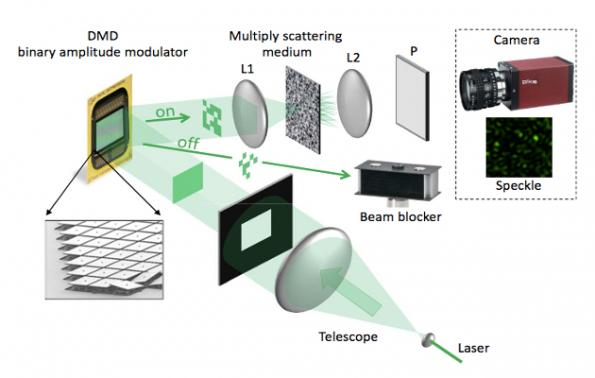
\includegraphics[scale=0.5]{figs/lighton630.jpg}
\end{center}
\caption[OPU's Experimental setup]{OPU's Experimental setup \citep{saade_opu}: A monochromatic laser is expanded by a telescope, then
illuminates a digital micromirror device (DMD), able to spatially encode digital information on the light beam by
amplitude modulation. The light beam carrying the signal is then focused on a random
medium by means of a lens. The transmitted light is collected on the
far side by a second lens, passes through a polarizer, and is measured by a standard monochrome CCD camera for example .}
\label{fig_opu}
\end{figure}
When the incident light is coherent, it promotes complex interference patterns, called speckles, due to the scattering process.
These speckles do not only characterize the propagation medium but also the incident light, and this can be modeled by $y=Wx$, 
where $y$ and $x$ are the vector amplitudes between a set of spatial modes at the output and at the input of the medium respectively. In OPUs, the transmission matrix $W$ of the propagation medium can be approximately considered to be a Gaussian i.i.d matrix. Although it is not explicitely known, it is guaranteed to be stable as long as the propagation medium is stable \citep{saade_opu}.  So using a spatial light modulator and a laser to send an appropriate set of illuminations to the propagation medium, we can acquire the output intensity $|y|^2$ with a CCD or CMOS camera, and that is the principle concept behind OPU's functionality as seen in Fig~ \ref{fig_opu}. To encode a given signal within the incident light, a OPU uses a DMD (digital micromirror device). It is a binary amplitude modulator consisting of an array of micro-mirrors. Each mirror can be activated or not, and thus represent a binary value. %In order to represent grey values, each value is encoded on a square sub-array ($4\times 4$ for example) in the DMD, where the number of lit mirrors reflects the desired level of grey. 
So, generally, a given signal $x$ must be encoded under the form of a binary vector before being passed to the OPU, however we remark that in our case, adjacency matrices of graphlets are already binary, which results in even more speed-up. %The DMD reflects the data and send the reflected light through the disordered medium, then a snapshot of the resulting random projection is acquired using a standard camera.

\subsection{Fast $GSA-\varphi_{OPU}$ algorithm}
One can efficiently deploy the random feature map $\varphi_{OPU}$ in the GSA-$\varphi$ framework, yielding the GSA-$\varphi_{OPU}$ algorithm : it is Algorithm~\ref{alg:GSA} where one uses the random projection $\varphi_{OPU}$ of Eq.~\eqref{OPU_equation} on the vectorized adjacency matrices of each sampled graphlet $F$.
%\begin{algorithm}[H]
%\DontPrintSemicolon
%  \KwInput{2-Classes labelled graph dataset $\mathcal{X}=(\G_i,y_i)_{i=1,\ldots,n}$}
%  \KwOutput{Trained model to classify graphs}
%  \tools{Graph random sampler $S_k$, optical processing unit (OPU), linear classifier (ex. SVM) }\\
%  \Hyp{k:graphlet size, $s$:\#graphlet samples per graph}\\
%  \Algo{\\}
%  Random initialization of the classifier weights\\
%  \For{$\G_i$ in $\mathcal{X}$}{
%  $\boldsymbol{\varphi}_{OPU}(i)=0$\\
%  \For{$j=1:s$}{
%  $F_{i,j}\gets S_k(\G_i)$\\
%  $\mathbf{A}\gets adjacency\_matrix(F_{i,j})$\\
%  $\boldsymbol{\varphi}_{OPU}(i)\gets \boldsymbol{\varphi}_{OPU}(i) +\frac{1}{s}\boldsymbol{\varphi}_{OPU}(F_{i,j})$
%  }
%  }
%  $\mathcal{D}_{\varphi_{OPU}}\gets (\boldsymbol{\varphi}_{OPU}(i),y_i)_{i=1,\ldots, n}$\\
%  Train the linear classifier on the new vector-valued dataset $\mathcal{D}_{\varphi_{OPU}}$
%\caption{GSA-$\varphi_{OPU}$}
%\end{algorithm}
%\todoNK{remove this algorithm}

As mentioned above, the computational cost of $\varphi_{OPU}$ is $\mathcal{O}(1)$, thus independent of both the number of random features and the graphlet size. One can reasonably argue that an OPU has its limits, as the DMD mirror array, where the input $\mathbf{A}$ is encrypted, has a limited dimensions \emph(width $\times$ length). Moreover, the camera used to acquire the light intensity in an OPU has a limited number of pixels thus it introduces a limit on the maximum number of random features. However, within these limits, which are usually large ones, the computational cost is a constant in both $m$ and $k$. 

%To better illustrate the advantage of $GSA-\varphi_{OPU}$ over other discussed methods in this work, we show a table comparing the various theoretical computational times in Table~\ref{table:comp_time}. 

%between them with respect to the computational time per graph $\G$:
%\begin{itemize}
%    \item Graphlet kernel: $C_{gk}= O(\tbinom{v}{k} N_k C_k)$
%    \item Graphlet kernel with sampling: $ C_{gk + gs}= O(C_S s N_k C_k)$
%    \item Gaussian features $GSA_{\varphi_{Gs}}$: $C_{Gs}=O(C_S smk^2)$
%    \item Gaussian features  $GSA_{\varphi_{Gs}}$ with Eigenvalue preprocessing: $C_{Gs+Eig}=O(C_S s(mk+k^3))$
%    \item $GSA_{\varphi_{OPU}}$:  $C_{OPU}=O(C_S s)$
%\end{itemize}

The complexities of the different mappings $\varphi$ examined in this work are summarized in Table \ref{tab:cost}.

\begin{table}
\centering
\begin{tabular}{|c|c|c|c|}
\hline
\multicolumn{2}{|c|}{Graphlet kernel} & \multicolumn{2}{|c|}{$O(\tbinom{v}{k} N_k C^{\cong}_k)$} \\ \hline \hline
%
\multirow{4}{*}{GSA-$\varphi$ with:} & Matching func. $\varphi^{match}_k$ & \multirow{4}{*}{$O(C_S s C_\varphi)$ with $C_\varphi=$ } & $O(N_k C^{\cong}_k)$ \\
& Gaussian RF & & $O(m k^2)$ \\ 
& Gaussian RF on Eig. & & $O(m k + k^3)$ \\ 
& OPU  & & $O(1)$ \\ \hline
\end{tabular}
\caption{Complexities of the different mappings used in GSA-$\varphi$, for a global cost in $O(C_S s C_ \varphi)$.}
\label{tab:cost}
\end{table}

\section{GSA-$\varphi$ concentration inequality proof}
\label{section:proof}

\begin{proof}
Here, we prove theorem \ref{theorem:concentration}. We decompose the proof in two steps.

\paragraph{Step 1: infinite $s$, finite $m$ (number of random features).} Based on our assumption $|\xi_w|\leq 1$, it is a straightforward result of Hoeffding's inequality that  $MMD(\G, \G')^2$ is close to $\frac{1}{m} \sum_{j=1} | \mathbb{E}_{F \sim S_k(\G)} \xi_{\mathbf{w}_j}(F) - \mathbb{E}_{F' \sim S_k(\G')} \xi_{\mathbf{w}_j}(F') |^2 = | \mathbb{E}_{F \sim S_k(\G)} \varphi(F) - \mathbb{E}_{F' \sim S_k(\G')} \varphi(F') |^2$. We recall Hoeffding's inequality below.
\begin{lemma}[Hoeffding's inequality] 
Let $(x_1,\ldots, x_m)$ be independent random variables such that the variable $x_i$ is strictly bounded by the interval $[a_i , b_i]$, and let $\overline{X}=\frac{1}{m}\Sigma_{i=1}^{m}x_i$ then we have:
\begin{equation}
\label{eq:Hoeffding}
    \mathbb{P}(|\mathbb{E}\overline{X}-\overline{X}|\geq \epsilon)\leq 2~ \exp \left(-\frac{2m^2\epsilon^2}{\Sigma_{i=1}^m(b_i-a_i)^2)} \right)
\end{equation}
\end{lemma}
%\begin
In our case, we define the variables $x_j=| \mathbb{E}_{F \sim S_k(\G)} \xi_{\mathbf{w}_j}(F) - \mathbb{E}_{F' \sim S_k(\G')} \xi_{\mathbf{w}_j}(F') |^2$. They are independent, have expectation $MMD(\G,\G')^2$, and are bounded by the interval $[0,4]$, thus we have:
\begin{equation*}
    \mathbb{P}\left(\Big|\frac{1}{m} \sum_{j=1}^m | \mathbb{E}_{F \sim S_k(\G)} \xi_{\mathbf{w}_j}(F) - \mathbb{E}_{F' \sim S_k(\G')} \xi_{\mathbf{w}_j}(F') |^2 - MMD(\G,\G')^2 \Big| \geq \epsilon\right) \leq 2~ e^{ -2m\epsilon^2/16}
\end{equation*}
Or, in other words, with probability $1-\delta$,
\begin{equation}\label{eq:step1}
\Big|\frac{1}{m} \sum_{j=1}^m | \mathbb{E}_{F \sim S_k(\G)} \xi_{\mathbf{w}_j}(F) - \mathbb{E}_{F' \sim S_k(\G')} \xi_{\mathbf{w}_j}(F') |^2 - MMD(\G,\G')^2 \Big| \leq \frac{4 \sqrt{\log (2/\delta)}}{\sqrt{m}}
\end{equation}

\paragraph{Step 2: finite ${s}$ and $m$.} We show that for any \emph{fixed} set of random features $\{\mathbf{w}_j\}$, we have $\| \mathbb{E}_{F \sim S_k(\G)} \varphi(F) - \mathbb{E}_{F' \sim S_k(\G')} \varphi(F')\|$ close to $\| \frac{1}{{s}} \sum_i \varphi(F_i) - \frac{1}{{s}} \sum_i \varphi(F'_i)\|$. 
%Let us consider a fixed set of random variables $\{\omega_j\}_{j \in \{1,\ldots, m\}}$ drawn independently from $\Lambda$, thus the random features map of a graph F equals: $z(F) = \frac{1}{\sqrt{m}}\left[z_{\omega_j}(F)\right]_{j=1}^m$.\newline
By definition of $F_1,\ldots, F_{s}$ random subgraphs drawn independently from $S_k(\G)$, we clearly have: 
\begin{equation}
\label{eq:subsample}
    \mathbb{E}_{F \sim S_k(\G)}~ \varphi(F)= \mathbb{E}\left(~\frac{1}{{s}} \sum_i \varphi(F_i)~\right)
\end{equation} 
Moreover by our assumptions $\varphi(F)$ is in a ball of radius $M=\frac{\sqrt{m}}{\sqrt{m}}=1$. We then apply the following vector version of Hoeffding's inequality.
\begin{lemma}
\label{lemma:vector_hoeffding}
let $X=\{x_1,\ldots,x_{s}\}$ be $iid$ random variables in a ball of radius $M$ centered around the origin in a Hilbert space $\mathcal{H}$. Denote their average by $\overline{X}=\frac{1}{{s}}\sum_{i=1}^{s}x_i$. Then for any $\delta>0$, with probability at lest $1-\delta$, 
\begin{equation}
\label{eq:vector_hoeffding0}
  \| \overline{X}-\mathbb{E}\overline{X}\|_\mathcal{H} \leq \frac{M}{\sqrt{{s}}}\left(1+\sqrt{2\log\frac{1}{\delta}}\right)
\end{equation}
\end{lemma}
\begin{proof}
Although this lemma is well-known in the literature, we reproduce its proof for completeness. Defining the function $f(x)= \| \overline{X}-\mathbb{E}\overline{X}\|$, and $\widetilde{X}={x_1,\ldots,\widetilde{x}_i,\ldots,x_{s}}$ to be a copy of $X$ with the ith element replaced by an arbitrary element of $\mathcal{H}$, we can prove using the triangle inequality:
\begin{equation}
    |f(X)-f(\widetilde{X})|=\Big|\| \overline{X}-\mathbb{E}\overline{X} \|-\|\overline{\widetilde{X}} - \mathbb{E}\overline{X}  \| \Big|\leq \| \overline{X} - \overline{\widetilde{X}}\|\leq
    \frac{\|x_i - \widetilde{x_i} \|}{{s}}\leq
    \frac{2M}{{s}}
\end{equation}
Therefore, $f(X)$ is insensitive to the ith component of $X,~ \forall i \in \{1,\ldots,{s}\}$ which suggests applying McDiarmid's inequality on $f$.

To bound the expectation of $f$, we use the familiar identity about the variance of the average of $iid$ random variables:
\begin{equation}
\mathbb{E}\|\overline{X}-\mathbb{E}\overline{X}\|^2=\frac{1}{n}(\mathbb{E}\|x\|^2-\|\mathbb{E}x\|^2 ) 
\end{equation}
Also:
\[ \mathbb{E}f(X)\leq\sqrt{\mathbb{E}f^2(X)}=\sqrt{\mathbb{E}\|\overline{X}-\mathbb{E}\overline{X}\|^2}\leq \frac{M}{\sqrt{{s}}}\]
This bound for the expectation of $f$ and McDiarmid's inequality give: 
\begin{equation}
\label{eq:vector_hoeffding1}
    \mathbb{P}_x \Big [ f(X)-\frac{M}{\sqrt{{s}}}\geq \epsilon \Big ]\leq
    \mathbb{P}_x \Big [ f(X)-\mathbb{E}f(X)\geq \epsilon \Big ]\leq
    \exp\Big( -\frac{{s}\epsilon^2}{2M^2}\Big)
\end{equation}
Which is equivalent to \eqref{eq:vector_hoeffding0} by setting $\delta=exp( -\frac{{s}\epsilon^2}{2M^2})$ and solving for $\epsilon$.
\end{proof}
Now back to Eq. \eqref{eq:subsample} and its corresponding assumptions that we made, we can directly apply lemma \ref{lemma:vector_hoeffding} (and more specifically Eq.~\eqref{eq:vector_hoeffding1}) to get that with probability $1-\delta$:
\begin{equation}
    \label{eq:fixed_w}
    \left\|\mathbb{E}_{F \sim S_k(\G)} \varphi(F)-~\frac{1}{s} \sum_i \varphi(F_i)~\right\|\geq \frac{1}{\sqrt{{s}}}\left(1+\sqrt{2\log\frac{1}{\delta}}\right)
\end{equation}
Now, by a union bound and triangle inequality: with probability $1-2\delta$,
\begin{align*}
    \Big | \| \mathbb{E}_{F \sim S_k(\G)} \varphi(F)& - \mathbb{E}_{F' \sim S_k(\G')} \varphi(F')\| - \| \frac{1}{{s}} \sum_i \varphi(F_i) - \frac{1}{{s}} \sum_i \varphi(F'_i)\|\Big | \\
    &\leq  \| \mathbb{E}_{F \sim S_k(\G)} \varphi(F) -  \frac{1}{{s}} \sum_i \varphi(F_i) \| + \|\mathbb{E}_{F' \sim S_k(\G')} \varphi(F') - \frac{1}{{s}} \sum_i \varphi(F'_i)\| \\
    &\leq \frac{2}{\sqrt{{s}}}\left(1+\sqrt{2\log\frac{1}{\delta}}\right)
\end{align*}
Moreover, since $\| \mathbb{E}_{F \sim S_k(\G)} \varphi(F)- \mathbb{E}_{F' \sim S_k(\G')} \varphi(F')\| + \| \frac{1}{{s}} \sum_i \varphi(F_i) - \frac{1}{{s}} \sum_i \varphi(F'_i)\| \leq 4$, with the same probability:
\begin{equation}\label{eq:step2}
    \Big | \| \mathbb{E}_{F \sim S_k(\G)} \varphi(F) - \mathbb{E}_{F' \sim S_k(\G')} \varphi(F')\|^2 - \| \frac{1}{{s}} \sum_i \varphi(F_i) - \frac{1}{{s}} \sum_i \varphi(F'_i)\|^2\Big | \leq \frac{8}{\sqrt{{s}}}\left(1+\sqrt{2\log\frac{1}{\delta}}\right)
\end{equation}
%Thus, since the two variables $\| \mathbb{E}_{F \sim f_G} z(F) -  \frac{1}{{s}} \sum_i z(F_i) \|$ and $\|\mathbb{E}_{F' \sim f_{G'}} z(F') - \frac{1}{{s}} \sum_i z(F'_i)\|$ are independent (as a direct result of our aforementioned assumption of independent random sampling), $\forall \epsilon>0$ we have:
%\begin{align*}
%    Pr( \| \mathbb{E}_{F \sim f_G} z(F) -  \frac{1}{{s}} \sum_i z(F_i) \| \geq \frac{1}{\sqrt{{s}}}+\frac{\epsilon}{2}, \|\mathbb{E}_{F' \sim f_{G'}} z(F') - \frac{1}{{s}} \sum_i z(F'_i)\|\geq\frac{1}{\sqrt{{s}}}+\frac{\epsilon}{2})=\\
%    Pr( \| \mathbb{E}_{F \sim f_G} z(F) -  \frac{1}{{s}} \sum_i z(F_i) \| \geq \frac{1}{\sqrt{{s}}}+\frac{\epsilon}{2})~Pr( \|\mathbb{E}_{F' \sim f_{G'}} z(F') - \frac{1}{{s}} \sum_i z(F'_i)\|\geq\frac{1}{\sqrt{{s}}}+\frac{\epsilon}{2})\leq 
%    e^{-\frac{{s}\epsilon^2}{4}}
%\end{align*}
%finally, we get as a straight result from above:
%\begin{align*}
%    Pr(\Big | \| \mathbb{E}_{F \sim f_G} z(F) - \mathbb{E}_{F' \sim f_{G'}} z(F')\| - \| \frac{1}{{s}} \sum_i z(F_i) - \frac{1}{{s}} \sum_i z(F'_i)\|\Big | \geq
%    \frac{2}{\sqrt{{s}}}+\epsilon)\leq e^{-\frac{n\epsilon^2}{4}}
%\end{align*}
%This is true for any fixed set of random variables  $\{w_j\}_{j \in \{1,\ldots, m\}}$ drawn independently from $p(w)$.
Since it is valid for any fixed set of random features, it is also valid with \emph{joint} probability on random features and samples, by the law of total probability.

Finally, combining \eqref{eq:step1}, \eqref{eq:step2}, a union bound and a triangular inequality, we have: with probability $1-3\delta$,
\begin{equation}
\Big|\|\varphi(\mathfrak{F}_\G) - \varphi(\mathfrak{F}_{\G'})\|^2 - MMD(\G,\G')^2 \Big| \leq \frac{4 \sqrt{\log (2/\delta)}}{\sqrt{m}} + \frac{8}{\sqrt{{s}}}\left(1+\sqrt{2\log\frac{1}{\delta}}\right)
\end{equation}
which concludes the proof by taking $\delta$ as $\delta/3$.

\end{proof}



%\include{chapter11/ch1}
%\include{chapter2/ch2}
%\include{chapter3/ch3}
%

\chapter{MATHEMATICS NOTATION}
\section{Some Math Stuff}
LaTeX{} has a special way to embed mathematical symbols and notations. Here are some of them. Also observe how a bullet list is made.
\begin{itemize}\itemsep0pt \parskip0pt \parsep0pt
\item greater than $\ge$
\item less than $\le$
\item percent sign \%
\item multiply $N\times N$
\item inline equation $M = N(N-1)/2$
\end{itemize}
Sed orci justo, rutrum in dolor a, consequat dictum mi. Sed luctus congue ex nec dignissim. Phasellus volutpat urna vestibulum ipsum vestibulum, quis venenatis justo consectetur. Nullam hendrerit nisl in rutrum convallis. Sed sit amet malesuada nisi. Phasellus dolor neque, vehicula vestibulum semper at, facilisis eget libero. Mauris interdum magna molestie, auctor felis a, condimentum odio. Pellentesque habitant morbi tristique senectus et netus et malesuada fames ac turpis egestas. Suspendisse maximus lacinia dignissim. Maecenas pharetra accumsan metus, sagittis dictum purus sollicitudin eget. Curabitur ut porttitor arcu, ut porttitor ipsum. Vestibulum porttitor finibus sapien, ac pharetra odio bibendum nec. Nullam tincidunt dignissim risus imperdiet dictum.

Pellentesque habitant morbi tristique senectus et netus et malesuada fames ac turpis egestas. Suspendisse maximus lacinia dignissim. Maecenas pharetra accumsan metus, sagittis dictum purus sollicitudin eget. Curabitur ut porttitor arcu, ut porttitor ipsum. Vestibulum porttitor finibus sapien, ac pharetra odio bibendum nec. Nullam tincidunt dignissim risus imperdiet dictum.
\section{Math equation}
Example of a mathematical formula:
\begin{equation}
  ADD = \sum_{i=1}^{M}|<D(n+1,i)>-<D(n,i)>|
  \label{add}
\end{equation}

Pellentesque habitant morbi tristique senectus et netus et malesuada fames ac turpis egestas. Suspendisse maximus lacinia dignissim. Maecenas pharetra accumsan metus, sagittis dictum purus sollicitudin eget. Curabitur ut porttitor arcu, ut porttitor ipsum. Vestibulum porttitor finibus sapien, ac pharetra odio bibendum nec. Nullam tincidunt dignissim risus imperdiet dictum.
\section{Chapter section}
Fusce ultricies pulvinar diam sed ultrices. Sed orci justo, rutrum in dolor a, consequat dictum mi. Sed luctus congue ex nec dignissim. Phasellus volutpat urna vestibulum ipsum vestibulum, quis venenatis justo consectetur. Nullam hendrerit nisl in rutrum convallis. Sed sit amet malesuada nisi. Phasellus dolor neque, vehicula vestibulum semper at, facilisis eget libero. Mauris interdum magna molestie, auctor felis a, condimentum odio. Pellentesque habitant morbi tristique senectus et netus et malesuada fames ac turpis egestas. Suspendisse maximus lacinia dignissim. Maecenas pharetra accumsan metus, sagittis dictum purus sollicitudin eget. Curabitur ut porttitor arcu, ut porttitor ipsum. Vestibulum porttitor finibus sapien, ac pharetra odio bibendum nec. Nullam tincidunt dignissim risus imperdiet dictum.

Pellentesque habitant morbi tristique senectus et netus et malesuada fames ac turpis egestas. Suspendisse maximus lacinia dignissim. Maecenas pharetra accumsan metus, sagittis dictum purus sollicitudin eget. Curabitur ut porttitor arcu, ut porttitor ipsum. Vestibulum porttitor finibus sapien, ac pharetra odio bibendum nec. Nullam tincidunt dignissim risus imperdiet dictum.

\section{Chapter section}
Fusce ultricies pulvinar diam sed ultrices. Sed orci justo, rutrum in dolor a, consequat dictum mi. Sed luctus congue ex nec dignissim. Phasellus volutpat urna vestibulum ipsum vestibulum, quis venenatis justo consectetur. Nullam hendrerit nisl in rutrum convallis. Sed sit amet malesuada nisi. Phasellus dolor neque, vehicula vestibulum semper at, facilisis eget libero. Mauris interdum magna molestie, auctor felis a, condimentum odio. Pellentesque habitant morbi tristique senectus et netus et malesuada fames ac turpis egestas. Suspendisse maximus lacinia dignissim. Maecenas pharetra accumsan metus, sagittis dictum purus sollicitudin eget. Curabitur ut porttitor arcu, ut porttitor ipsum. Vestibulum porttitor finibus sapien, ac pharetra odio bibendum nec. Nullam tincidunt dignissim risus imperdiet dictum.

Pellentesque habitant morbi tristique senectus et netus et malesuada fames ac turpis egestas. Suspendisse maximus lacinia dignissim. Maecenas pharetra accumsan metus, sagittis dictum purus sollicitudin eget. Curabitur ut porttitor arcu, ut porttitor ipsum. Vestibulum porttitor finibus sapien, ac pharetra odio bibendum nec. Nullam tincidunt dignissim risus imperdiet dictum.

\chapter{FIGURES AND TABLES}
\section{Examples of a figure}
Fusce ultricies pulvinar diam sed ultrices. Sed orci justo, rutrum in dolor a, consequat dictum mi. Sed luctus congue ex nec dignissim. Phasellus volutpat urna vestibulum ipsum vestibulum, quis venenatis justo consectetur. Nullam hendrerit nisl in rutrum convallis. Sed sit amet malesuada nisi.

Example of a figure.
\begin{figure}[ht!]
\begin{center}
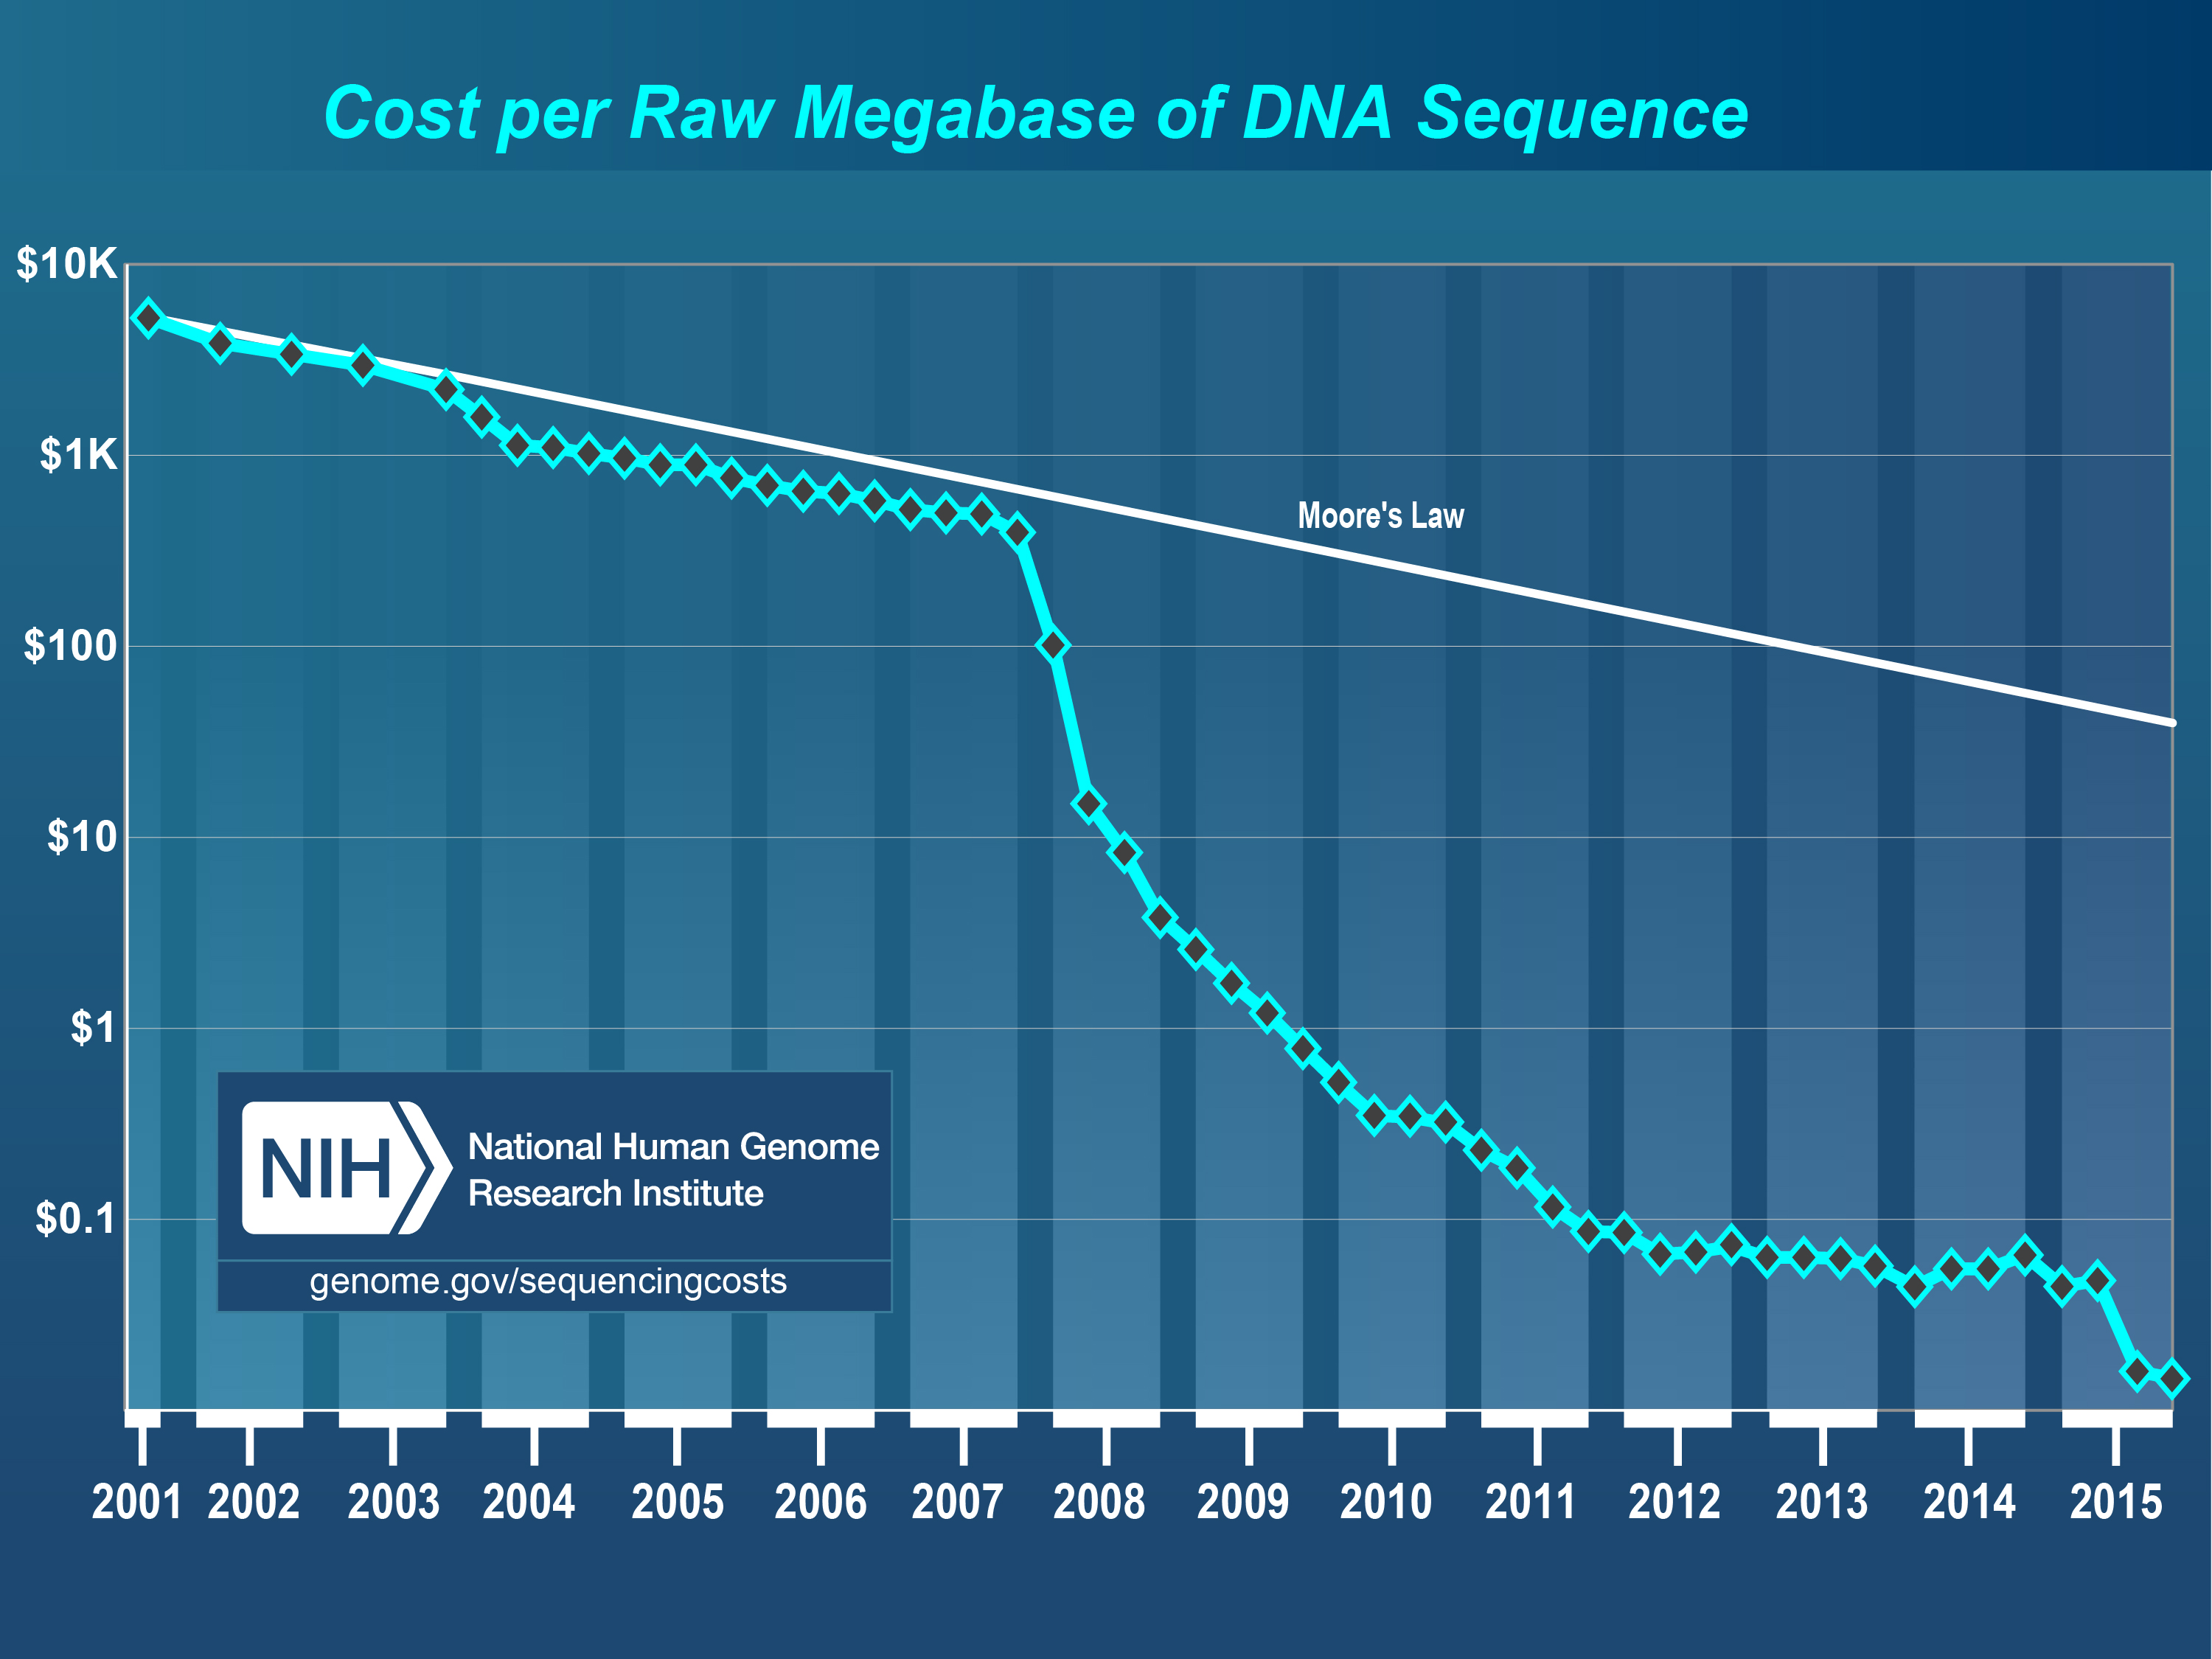
\includegraphics[scale=0.5]{costperMb2015_4.jpg}
\end{center}
\caption[Cost per raw megabase of DNA sequence from 2001 to 2015]{Cost per raw megabase of DNA sequence from 2001 to 2015. Straight line - Moore's Law, blue curve - cost in US dollars, Y-axis scale is logarithmic. Graph reproduced from \citep{wetterstrand2016}}
%Source:
\label{fig_dna_cost}
\end{figure}
Example of reference to a figure in the text (Fig.~\ref{fig_dna_cost}). Phasellus dolor neque, vehicula vestibulum semper at, facilisis eget libero. Mauris interdum magna molestie, auctor felis a, condimentum odio. Pellentesque habitant morbi tristique senectus et netus et malesuada fames ac turpis egestas. Suspendisse maximus lacinia dignissim. Maecenas pharetra accumsan metus, sagittis dictum purus sollicitudin eget. Curabitur ut porttitor arcu, ut porttitor ipsum. Vestibulum porttitor finibus sapien, ac pharetra odio bibendum nec. Nullam tincidunt dignissim risus imperdiet dictum.

Pellentesque habitant morbi tristique senectus et netus et malesuada fames ac turpis egestas. Suspendisse maximus lacinia dignissim. Maecenas pharetra accumsan metus, sagittis dictum purus sollicitudin eget. Curabitur ut porttitor arcu, ut porttitor ipsum. Vestibulum porttitor finibus sapien, ac pharetra odio bibendum nec. Nullam tincidunt dignissim risus imperdiet dictum.
\section{Example of a table}
Example of a table and here is the reference to Table \ref{table_genomes}. Tables in, my opinion, are the hardest thing to make.

\begin{table}
\begin{center}
\begin{tabular}{|l|c|c|c|}
\hline
{\sc Organism}  &  {\sc Accession no.}  & {\sc Genome size} (bp)  & {\sc No. CDS} \\
\hline
{\it Mesorhizobium loti}          & NC\_002678 & 7036071 & 6743 \\
\hline
{\it Sinorhizobium meliloti}      & NC\_003047 & 3654135 & 3359 \\
\hline
{\it Bradyrhizobium japonicum}    & NC\_004463 & 9105828 & 8317 \\
\hline
{\it Rhodopseudomonas palustris}  & NC\_005296 & 5459213 & 4813 \\
\hline
{\it Bartonella quintana}         & NC\_005955 & 1581384 & 1142 \\
\hline
{\it Bartonella henselae}         & NC\_005956 & 1931047 & 1488 \\
\hline
{\it Rickettsia typhi}            & NC\_006142 & 1111496 & 837 \\
\hline
{\it Beijerinckia indica}         & NC\_010581 & 4170153 & 3569 \\
\hline
\end{tabular}
\end{center}
\caption{Whole-genome sequences used in this study}
\label{table_genomes}
\end{table}

Fusce ultricies pulvinar diam sed ultrices. Sed orci justo, rutrum in dolor a, consequat dictum mi. Sed luctus congue ex nec dignissim. Phasellus volutpat urna vestibulum ipsum vestibulum, quis venenatis justo consectetur. Nullam hendrerit nisl in rutrum convallis. Sed sit amet malesuada nisi. Phasellus dolor neque, vehicula vestibulum semper at, facilisis eget libero. Mauris interdum magna molestie, auctor felis a, condimentum odio. Pellentesque habitant morbi tristique senectus et netus et malesuada fames ac turpis egestas. Suspendisse maximus lacinia dignissim. Maecenas pharetra accumsan metus, sagittis dictum purus sollicitudin eget. Curabitur ut porttitor arcu, ut porttitor ipsum. Vestibulum porttitor finibus sapien, ac pharetra odio bibendum nec. Nullam tincidunt dignissim risus imperdiet dictum.

Pellentesque habitant morbi tristique senectus et netus et malesuada fames ac turpis egestas. Suspendisse maximus lacinia dignissim. Maecenas pharetra accumsan metus, sagittis dictum purus sollicitudin eget. Curabitur ut porttitor arcu, ut porttitor ipsum. Vestibulum porttitor finibus sapien, ac pharetra odio bibendum nec. Nullam tincidunt dignissim risus imperdiet dictum.
\section{Chapter section}
Fusce ultricies pulvinar diam sed ultrices. Sed orci justo, rutrum in dolor a, consequat dictum mi. Sed luctus congue ex nec dignissim. Phasellus volutpat urna vestibulum ipsum vestibulum, quis venenatis justo consectetur. Nullam hendrerit nisl in rutrum convallis. Sed sit amet malesuada nisi. Phasellus dolor neque, vehicula vestibulum semper at, facilisis eget libero. Mauris interdum magna molestie, auctor felis a, condimentum odio. Pellentesque habitant morbi tristique senectus et netus et malesuada fames ac turpis egestas. Suspendisse maximus lacinia dignissim. Maecenas pharetra accumsan metus, sagittis dictum purus sollicitudin eget. Curabitur ut porttitor arcu, ut porttitor ipsum. Vestibulum porttitor finibus sapien, ac pharetra odio bibendum nec. Nullam tincidunt dignissim risus imperdiet dictum.

Pellentesque habitant morbi tristique senectus et netus et malesuada fames ac turpis egestas. Suspendisse maximus lacinia dignissim. Maecenas pharetra accumsan metus, sagittis dictum purus sollicitudin eget. Curabitur ut porttitor arcu, ut porttitor ipsum. Vestibulum porttitor finibus sapien, ac pharetra odio bibendum nec. Nullam tincidunt dignissim risus imperdiet dictum.


% Bibliography
\begingroup
    \setlength\bibitemsep{10pt}
    \linespread{1}\selectfont
    \printbibliography[title=REFERENCES]
\endgroup
\addcontentsline{toc}{part}{REFERENCES}

% Appendices
%\begin{appendices}
\section{Proof of Theorem 1}\label{app:proof}
\begin{proof} We decompose the proof in two steps.

\textbf{Step 1: infinite $s$, finite $m$.} First we define the random variables $x_j=| \mathbb{E}_{F \sim S_k(\G)} \xi_{\mathbf{w}_j}(F) - \mathbb{E}_{F' \sim S_k(\G')} \xi_{\mathbf{w}_j}(F') |^2$, which are: i/independent, ii/have expectation $MMD(\G,\G')^2$, /iii are bounded by the interval $[0,4]$ based on our assumption $|\xi_w|\leq 1$. Thus, as a straight result of applying  Hoeffding's inequality with easy manipulation: with probability $1-\delta$
\begin{equation}
\label{eq:step1}
\Big|\frac{1}{m} \sum_{j=1}^m x_j- MMD(\G,\G')^2 \Big| \leq\\ \frac{4 \sqrt{\log (2/\delta)}}{\sqrt{m}}
\end{equation}

\textbf{Step 2: finite $s$ and $m$.} For any \emph{fixed} set of random features $\{w_j\}_{1,\ldots,m}$ and based on our previous assumptions we have: i/ $\varphi_{RF}$ is in a ball of radius $M=\frac{\sqrt{m}}{\sqrt{m}}=1$, ii/ $ \mathbb{E}_{F \sim S_k(\G)}~ \varphi(F)= \mathbb{E}\left(~\frac{1}{{s}} \sum_i \varphi(F_i)~\right)$. Therefore, we can directly apply the vector version of Hoeffding's inequality on the vectors $\frac{1}{{s}} \sum_i \varphi(F_i)$ to get that with probability $1-\delta$:
\begin{equation}
    \label{eq:fixed_w}
    \left\|\mathbb{E}_{F \sim S_k(\G)} \varphi(F)-~\frac{1}{s} \sum_i \varphi(F_i)~\right\|\leq \frac{1+\sqrt{2\log\frac{1}{\delta}}}{\sqrt{{s}}}
\end{equation}
\vfill\pagebreak
Defining $J_{exp}(\G,\G')=\| \mathbb{E}_{F \sim S_k(\G)} \varphi(F) - \mathbb{E}_{F' \sim S_k(\G')} \varphi(F')\|$ and $J_{avg}(\G,\G')=\| \frac{1}{{s}} \sum_i \varphi(F_i) - \frac{1}{{s}} \sum_i \varphi(F'_i)\|$, then using triangular inequality followed by a union bound based on \eqref{eq:fixed_w}, we have the following with probability $1-2\delta$,
\begin{align*}
    \Big | J_{exp}(\G,\G') - J_{avg}(\G,\G')\Big | \leq \frac{2}{\sqrt{{s}}}\left(1+\sqrt{2\log\frac{1}{\delta}}\right)
\end{align*}

On the other hand, $ J_{exp}(\G,\G') + J_{avg}(\G,\G')\leq 4$, so with same probability:
\begin{equation}\label{eq:step2}
    \Big | J_{exp}(\G,\G')^2 - J_{avg}(\G,\G')^2 \Big | \leq \frac{8}{\sqrt{{s}}}\left(1+\sqrt{2\log\frac{1}{\delta}}\right)
\end{equation}
Since it is valid for any fixed set of random features, it is also valid with \emph{joint} probability on random features and samples, by the law of total probability.

Finally, combining \eqref{eq:step1}, \eqref{eq:step2} with a union bound and a triangular inequality, we have with probability $1-3\delta$,
\begin{align*}
\Big|\|\varphi(\mathfrak{F}_\G) - \varphi(\mathfrak{F}_{\G'})\|^2 - MMD(\G,\G')^2 \Big| \leq \\\frac{4 \sqrt{\log (2/\delta)}}{\sqrt{m}} + \frac{8}{\sqrt{{s}}}\left(1+\sqrt{2\log\frac{1}{\delta}}\right)
\end{align*}

which concludes the proof by taking $\delta$ as $\delta/3$.

\end{proof}
\end{appendices}

\end{document}
